%%%%%%from Rmarkdown%%%%%%
% Options for packages loaded elsewhere
\PassOptionsToPackage{unicode}{hyperref}
\PassOptionsToPackage{hyphens}{url}
%
%%%%%%from Rmarkdown%%%%%%
\documentclass[12pt]{article}

\usepackage[margin=1in]{geometry}
	%changes default margins
\usepackage{subcaption} %subfigure
\usepackage{setspace}
\usepackage{multirow}
\usepackage{booktabs}
\doublespacing
	%\singlespacing,\onehalfspacing,\doublespacing can be set and everything thereafter will use that spacing. You can switch within the document as often as you wish
	
\usepackage{parskip}
%changes paragraphs to have an extra space and new indentation with paragraphs, rather than indenting every new paragraph. This is completely a stylistic choice and neither is better than the other.


\usepackage{mathtools,amssymb} %useful math stuff. there are a lot of ams* packages. If you have a math need, it's probably in there

	
	
%\usepackage{natbib}
%\usepackage{biblatex} %natbib is older and available from almost all journals, biblatex is not, but biblatex has more flexibility and options.

%\usepackage[natbib=true]{biblatex} %this often works and requires minimal changes 

%for biblatex you write \textcite{citekey} and \parencite{citekey}
%for natbib you write \citet{citekey} and \citep{citekey}. Please avoid using \cite{} since you won't control whether it's parenthetical, but you are responsible for whether you use something in text or parenthetically.
%for \usepackage[natbib=true]{biblatex} you follow the natbib style and you won't have to perform search/replaces in your document, you would only need to change the package call and bibliography call.

\usepackage{natbib}
\bibliographystyle{chicago}

%other useful packages
% \usepackage{graphicx} %for including images including pdf

%%%%%%from Rmarkdown%%%%%%
\usepackage{iftex}
\ifPDFTeX
  \usepackage[T1]{fontenc}
  \usepackage[utf8]{inputenc}
  \usepackage{textcomp} % provide euro and other symbols
\else % if luatex or xetex
  \usepackage{unicode-math} % this also loads fontspec
  \defaultfontfeatures{Scale=MatchLowercase}
  \defaultfontfeatures[\rmfamily]{Ligatures=TeX,Scale=1}
\fi
\usepackage{lmodern}
\ifPDFTeX\else
  % xetex/luatex font selection
\fi
% Use upquote if available, for straight quotes in verbatim environments
\IfFileExists{upquote.sty}{\usepackage{upquote}}{}
\IfFileExists{microtype.sty}{% use microtype if available
  \usepackage[]{microtype}
  \UseMicrotypeSet[protrusion]{basicmath} % disable protrusion for tt fonts
}{}
\makeatletter
\@ifundefined{KOMAClassName}{% if non-KOMA class
  \IfFileExists{parskip.sty}{%
    \usepackage{parskip}
  }{% else
    \setlength{\parindent}{0pt}
    \setlength{\parskip}{6pt plus 2pt minus 1pt}}
}{% if KOMA class
  \KOMAoptions{parskip=half}}
\makeatother
\usepackage{xcolor}
\usepackage[margin=1in]{geometry}
\usepackage{color}
\usepackage{fancyvrb}
\newcommand{\VerbBar}{|}
\newcommand{\VERB}{\Verb[commandchars=\\\{\}]}
\DefineVerbatimEnvironment{Highlighting}{Verbatim}{commandchars=\\\{\}}
% Add ',fontsize=\small' for more characters per line
\usepackage{framed}
\definecolor{shadecolor}{RGB}{248,248,248}
\newenvironment{Shaded}{\begin{snugshade}}{\end{snugshade}}
\newcommand{\AlertTok}[1]{\textcolor[rgb]{0.94,0.16,0.16}{#1}}
\newcommand{\AnnotationTok}[1]{\textcolor[rgb]{0.56,0.35,0.01}{\textbf{\textit{#1}}}}
\newcommand{\AttributeTok}[1]{\textcolor[rgb]{0.13,0.29,0.53}{#1}}
\newcommand{\BaseNTok}[1]{\textcolor[rgb]{0.00,0.00,0.81}{#1}}
\newcommand{\BuiltInTok}[1]{#1}
\newcommand{\CharTok}[1]{\textcolor[rgb]{0.31,0.60,0.02}{#1}}
\newcommand{\CommentTok}[1]{\textcolor[rgb]{0.56,0.35,0.01}{\textit{#1}}}
\newcommand{\CommentVarTok}[1]{\textcolor[rgb]{0.56,0.35,0.01}{\textbf{\textit{#1}}}}
\newcommand{\ConstantTok}[1]{\textcolor[rgb]{0.56,0.35,0.01}{#1}}
\newcommand{\ControlFlowTok}[1]{\textcolor[rgb]{0.13,0.29,0.53}{\textbf{#1}}}
\newcommand{\DataTypeTok}[1]{\textcolor[rgb]{0.13,0.29,0.53}{#1}}
\newcommand{\DecValTok}[1]{\textcolor[rgb]{0.00,0.00,0.81}{#1}}
\newcommand{\DocumentationTok}[1]{\textcolor[rgb]{0.56,0.35,0.01}{\textbf{\textit{#1}}}}
\newcommand{\ErrorTok}[1]{\textcolor[rgb]{0.64,0.00,0.00}{\textbf{#1}}}
\newcommand{\ExtensionTok}[1]{#1}
\newcommand{\FloatTok}[1]{\textcolor[rgb]{0.00,0.00,0.81}{#1}}
\newcommand{\FunctionTok}[1]{\textcolor[rgb]{0.13,0.29,0.53}{\textbf{#1}}}
\newcommand{\ImportTok}[1]{#1}
\newcommand{\InformationTok}[1]{\textcolor[rgb]{0.56,0.35,0.01}{\textbf{\textit{#1}}}}
\newcommand{\KeywordTok}[1]{\textcolor[rgb]{0.13,0.29,0.53}{\textbf{#1}}}
\newcommand{\NormalTok}[1]{#1}
\newcommand{\OperatorTok}[1]{\textcolor[rgb]{0.81,0.36,0.00}{\textbf{#1}}}
\newcommand{\OtherTok}[1]{\textcolor[rgb]{0.56,0.35,0.01}{#1}}
\newcommand{\PreprocessorTok}[1]{\textcolor[rgb]{0.56,0.35,0.01}{\textit{#1}}}
\newcommand{\RegionMarkerTok}[1]{#1}
\newcommand{\SpecialCharTok}[1]{\textcolor[rgb]{0.81,0.36,0.00}{\textbf{#1}}}
\newcommand{\SpecialStringTok}[1]{\textcolor[rgb]{0.31,0.60,0.02}{#1}}
\newcommand{\StringTok}[1]{\textcolor[rgb]{0.31,0.60,0.02}{#1}}
\newcommand{\VariableTok}[1]{\textcolor[rgb]{0.00,0.00,0.00}{#1}}
\newcommand{\VerbatimStringTok}[1]{\textcolor[rgb]{0.31,0.60,0.02}{#1}}
\newcommand{\WarningTok}[1]{\textcolor[rgb]{0.56,0.35,0.01}{\textbf{\textit{#1}}}}
\usepackage{graphicx}
\makeatletter
\def\maxwidth{\ifdim\Gin@nat@width>\linewidth\linewidth\else\Gin@nat@width\fi}
\def\maxheight{\ifdim\Gin@nat@height>\textheight\textheight\else\Gin@nat@height\fi}
\makeatother
% Scale images if necessary, so that they will not overflow the page
% margins by default, and it is still possible to overwrite the defaults
% using explicit options in \includegraphics[width, height, ...]{}
\setkeys{Gin}{width=\maxwidth,height=\maxheight,keepaspectratio}
% Set default figure placement to htbp
\makeatletter
\def\fps@figure{htbp}
\makeatother
\setlength{\emergencystretch}{3em} % prevent overfull lines
\providecommand{\tightlist}{%
  \setlength{\itemsep}{0pt}\setlength{\parskip}{0pt}}
\setcounter{secnumdepth}{-\maxdimen} % remove section numbering
\ifLuaTeX
  \usepackage{selnolig}  % disable illegal ligatures
\fi
\IfFileExists{bookmark.sty}{\usepackage{bookmark}}{\usepackage{hyperref}}
\IfFileExists{xurl.sty}{\usepackage{xurl}}{} % add URL line breaks if available
\urlstyle{same}
%%%%%%from Rmarkdown%%%%%%

\title{Ast3: Death's End}
%\author{jsp ci 843503,\\ 
%	eswst i; ,i;l 830097,\\ 
%sjsms ,ovjs; 839866}
\author{
Hao Xu T00732492,\\
Waqar Ul Mulk T00729986,\\
Ahana Michael T00728755}
\date{\today}

\begin{document}
	
\maketitle

\section{Question 1}

\textbf{Because your response is binary (0 or 1), and you are modelling its expected value, what is your kernel smoother actually modelling? Hint: one of two words, both of which start with p.}

\underline{Probability}

\[
P(\text{isGentoo}=1 \mid \mathbf{x}_0) = \hat{f}(\mathbf{x}_0) = \frac{\sum_{i=1}^{N} K_{Type, \lambda}\left( \mathbf{x}_0, \mathbf{x}_i \right) y_i}{\sum_{i=1}^{N} K_{Type,\lambda}\left( \mathbf{x}_0, \mathbf{x}_i \right)}
\] 

Where $\mathbf{x}_0$ is a new data point in the test dataset, $N$ is the size of training data set, $K_{Type, \lambda}$ is the kernel function, and $\lambda$ is the bandwidth, $y_i$ represent the label of the $i^{\text{th}}$ training data.

\section{Question 2}

We implemented 2 different types of kernels: Box and Triangle. 

\begin{align*}
K_{\text{Box}, \lambda}(\mathbf{x}_0, \mathbf{x}_i) &= 
\begin{cases}
1, &\quad d_{*}(\mathbf{x}_0, \mathbf{x}_i)<\lambda\\
0, &\quad \text{otherwise}\\
\end{cases}\\
K_{\text{Triangle}, \lambda}(\mathbf{x}_0, \mathbf{x}_i) &= 
\begin{cases}
\frac{\lambda - d_{*}(\mathbf{x}_0, \mathbf{x}_i)}{\lambda}, &\quad d_{*}(\mathbf{x}_0, \mathbf{x}_i)<\lambda\\
0, &\quad \text{otherwise}\\
\end{cases}
\end{align*}

Where $d_{*}$ represent different types of distance metric: $d_{*} = d_{1}$ represent the $L_1$ (Manhattan) distance and $d_{*} = d_{2}$ represent the $L_2$ (Euclidean) distance.

%$L_1$ (Manhattan) distance between $\mathbf{a}=(a_1,a_2,a_3,a_4)$ and $\mathbf{b}=(b_1,b_2,b_3,b_4)$:
%\[
%d_{1}(\mathbf{a},\mathbf{b})=|a_1-b_1|+|a_2-b_2|+|a_3-b_3|+|a_4-b_4|
%.\] 
%
%$d_{*} = d_{2}$ represent the $L_2$ (Euclidean) distance between $\mathbf{a}=(a_1,a_2,a_3,a_4)$ and $\mathbf{b}=(b_1,b_2,b_3,b_4)$:
%\[
%d_{2}(\mathbf{a},\mathbf{b})=\sqrt{\left( a_1-b_1 \right) ^2+\left( a_2-b_2 \right) ^2+\left( a_3-b_3 \right) ^{2}+\left( a_4-b_4 \right) ^{2}} 
%.\] 

The output of our model is as follows:
\[
\text{Prediction}(\mathbf{x}_0)= 
\begin{cases}
1, &\quad P(\text{isGentoo}=1 \mid \mathbf{x}_0) = \hat{f}(\mathbf{x}_0) \ge 0.5\\
0, &\quad \text{otherwise}\\
\end{cases}
\]
If the probability of $\mathbf{x}_0$ to be Gentoo is greater than 50\%, we say it is Gentoo. \footnote{Here, this 50\% threshhold is arbitrarily selected. Theoratically, this threshhold can be any value in $\left( 0,1 \right) $ because we can use $\lambda$ to control the number of data points we included in our kernel. A lower threshold will result in a smaller $\lambda$ to get the best accuracy, vice versa.}

Not creating a training/test partition is a bad idea because we can always use a very small $\lambda$ to achieve 100\% training accuracy\footnote{This is because no matter how unreasonably small the $\lambda$ is, we always have one correct data point $\mathbf{x}_0$ selected by our kernel.}. Therefore, we use 10-fold cross validation to train and test our data. We define our training score as the average of test error rates across all 10 folds as follows: ($N_i$ is the $i^{\text{th}}$ test partition)
\[
\text{ERROR}_{Type,\lambda,d} = \left(\sum_{i=1}^{10}  \frac{\sum_{j\in N_i} \text{err}(j)}{|N_i|} \right) \cdot \frac{1}{10}, \quad \text{err}(j)=
\begin{cases}
1, &\quad \text{Prediction}\left(\mathbf{x}_j \right) \neq y_j\\
0, &\quad \text{otherwise}\\
\end{cases}\\
\] 

\begin{figure}[htbp]
\centering
\begin{subfigure}{0.6\textwidth}
    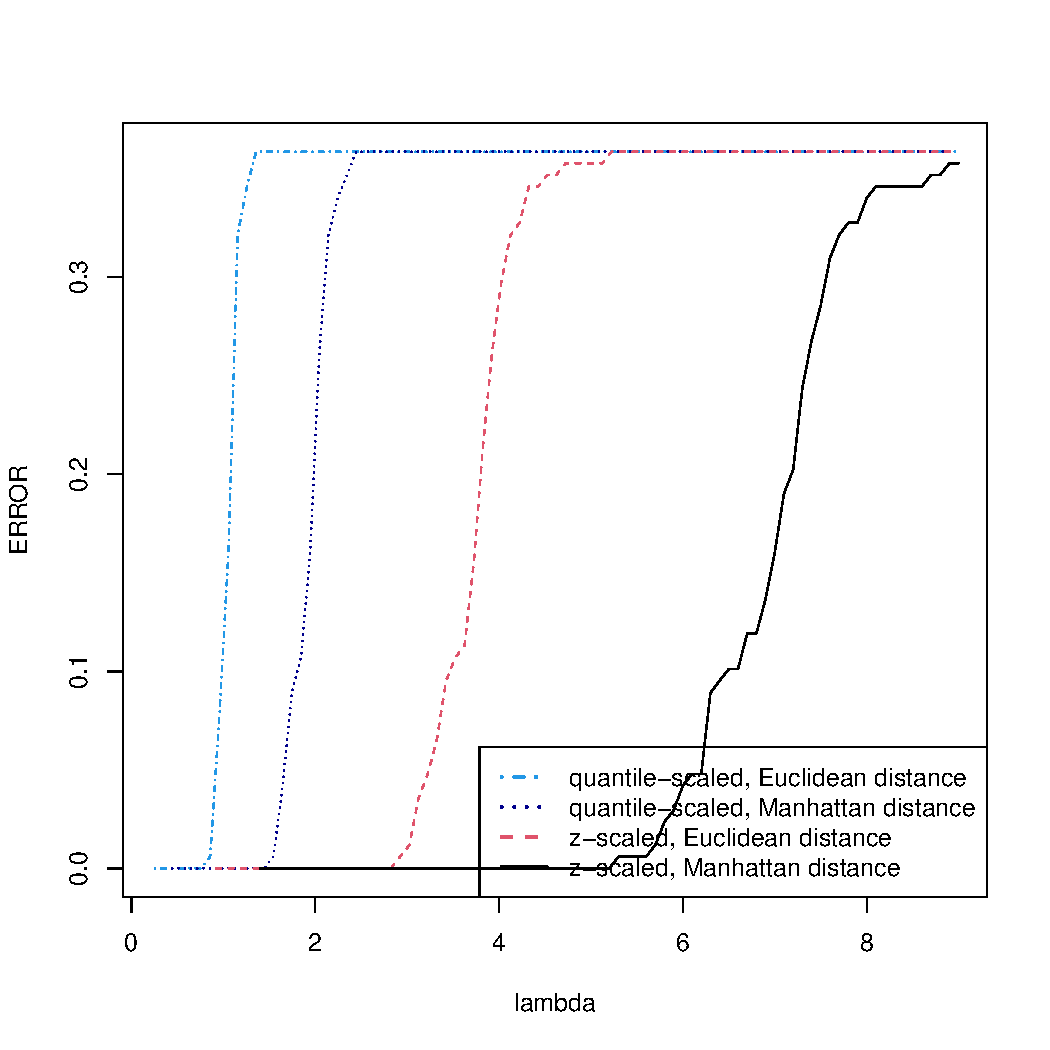
\includegraphics[width=\textwidth]{ERROR-lambda}
    \caption{Box Kernel}
    \label{fig:first}
\end{subfigure}
\hfill
\begin{subfigure}{0.6\textwidth}
    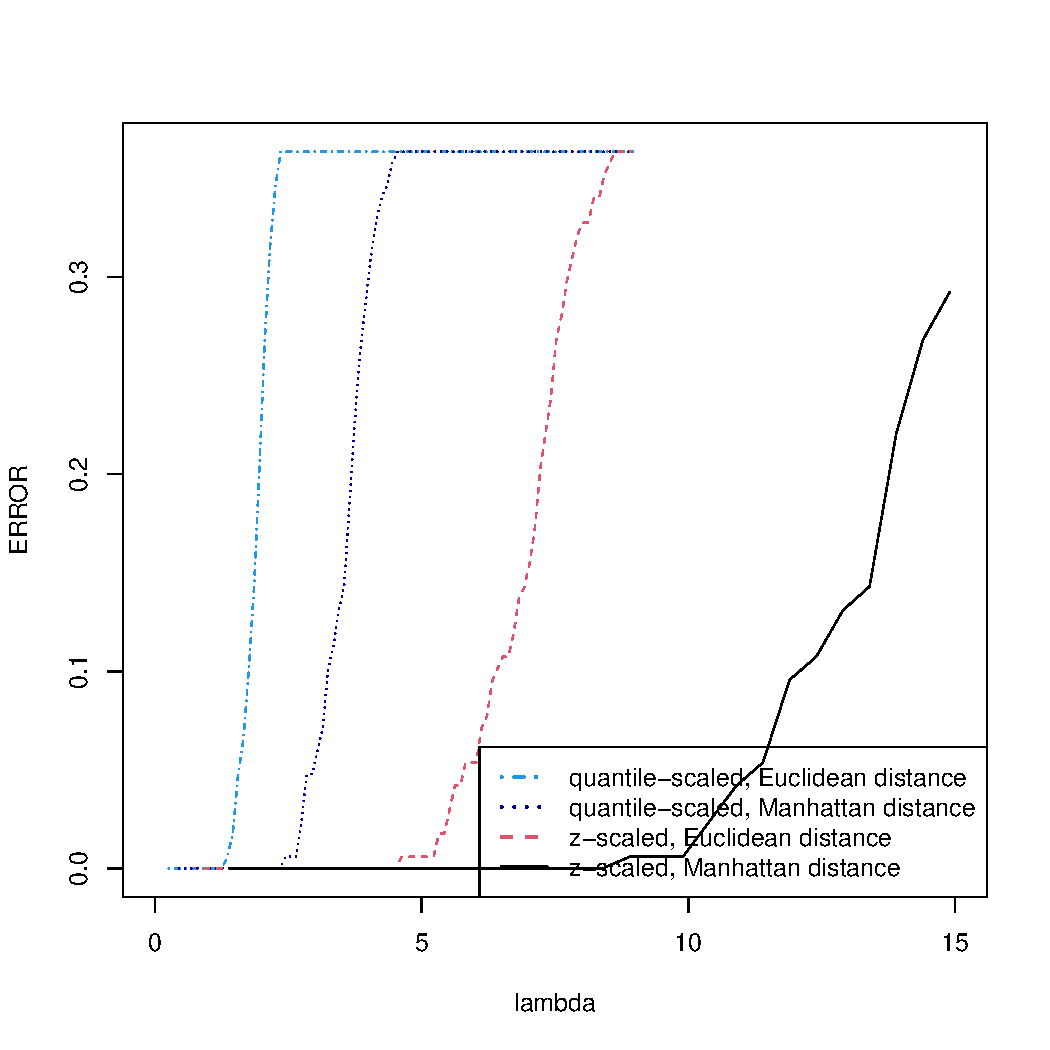
\includegraphics[width=\textwidth]{ERROR-lambda2}
    \caption{Triangle Kernel}
    \label{fig:second}
\end{subfigure}
        
\caption{ERROR-$\lambda$ plot}
\label{fig:result}
\end{figure}

The average test error rates depends on (1) the kernel bandwidth $\lambda$, (2) the type of distance metric and (3) the type of Kernel. Figure~\ref{fig:result} plots the ERROR--$\lambda$ relation. Box Kernel is used in figure~\ref{fig:first} and Triangle Kernel is used in figure~\ref{fig:second}. Comparing those figures, we can see that quantile scaled data requires a smaller $\lambda$, whereas z-scored scaled data requires a relative larger $\lambda$. Also Manhattan distance metric requires a relative larger $\lambda$ compares to Euclidean distance.

Additionally, we can see that Triangle Kernel performs more stable than Box Kernel (More tolerance to changes in $\lambda$).

\newpage
\section{Appendix: Code}

\begin{Shaded}
\begin{Highlighting}[]
\FunctionTok{library}\NormalTok{(palmerpenguins)}
\CommentTok{\# Select the male penguins}
\NormalTok{mpenguins }\OtherTok{\textless{}{-}}\NormalTok{ penguins[}\FunctionTok{which}\NormalTok{(penguins}\SpecialCharTok{$}\NormalTok{sex }\SpecialCharTok{==} \StringTok{"male"}\NormalTok{),]}
\CommentTok{\# Add a new variable isGentoo}
\NormalTok{mpenguins}\SpecialCharTok{$}\NormalTok{isGentoo }\OtherTok{\textless{}{-}}\NormalTok{ mpenguins}\SpecialCharTok{$}\NormalTok{species }\SpecialCharTok{==} \StringTok{"Gentoo"}

\CommentTok{\# Using z{-}scores on each of the variables before applying distances}
\NormalTok{zscale }\OtherTok{\textless{}{-}} \ControlFlowTok{function}\NormalTok{(datacol)\{}
\NormalTok{mu }\OtherTok{\textless{}{-}} \FunctionTok{mean}\NormalTok{(datacol)}
\NormalTok{sigma }\OtherTok{\textless{}{-}} \FunctionTok{sd}\NormalTok{(datacol)}
\NormalTok{result }\OtherTok{\textless{}{-}}\NormalTok{ (datacol}\SpecialCharTok{{-}}\NormalTok{mu)}\SpecialCharTok{/}\NormalTok{sigma}
\FunctionTok{return}\NormalTok{(result)}
\NormalTok{\}}
\NormalTok{mpenguins}\SpecialCharTok{$}\NormalTok{zflipper\_length\_mm }\OtherTok{\textless{}{-}} \FunctionTok{zscale}\NormalTok{(mpenguins}\SpecialCharTok{$}\NormalTok{flipper\_length\_mm)}
\NormalTok{mpenguins}\SpecialCharTok{$}\NormalTok{zbill\_depth\_mm }\OtherTok{\textless{}{-}} \FunctionTok{zscale}\NormalTok{(mpenguins}\SpecialCharTok{$}\NormalTok{bill\_depth\_mm)}
\NormalTok{mpenguins}\SpecialCharTok{$}\NormalTok{zbill\_length\_mm }\OtherTok{\textless{}{-}} \FunctionTok{zscale}\NormalTok{(mpenguins}\SpecialCharTok{$}\NormalTok{bill\_length\_mm)}
\NormalTok{mpenguins}\SpecialCharTok{$}\NormalTok{zbody\_mass\_g }\OtherTok{\textless{}{-}} \FunctionTok{zscale}\NormalTok{(mpenguins}\SpecialCharTok{$}\NormalTok{body\_mass\_g)}

\CommentTok{\# Turning all (univariate) variables into quantiles}
\NormalTok{qscale }\OtherTok{\textless{}{-}} \ControlFlowTok{function}\NormalTok{(datacol)\{}
\FunctionTok{return}\NormalTok{(}\FunctionTok{ecdf}\NormalTok{(datacol)(datacol))}
\NormalTok{\}}
\NormalTok{mpenguins}\SpecialCharTok{$}\NormalTok{qflipper\_length\_mm }\OtherTok{\textless{}{-}} \FunctionTok{qscale}\NormalTok{(mpenguins}\SpecialCharTok{$}\NormalTok{flipper\_length\_mm)}
\NormalTok{mpenguins}\SpecialCharTok{$}\NormalTok{qbill\_depth\_mm }\OtherTok{\textless{}{-}} \FunctionTok{qscale}\NormalTok{(mpenguins}\SpecialCharTok{$}\NormalTok{bill\_depth\_mm)}
\NormalTok{mpenguins}\SpecialCharTok{$}\NormalTok{qbill\_length\_mm }\OtherTok{\textless{}{-}} \FunctionTok{qscale}\NormalTok{(mpenguins}\SpecialCharTok{$}\NormalTok{bill\_length\_mm)}
\NormalTok{mpenguins}\SpecialCharTok{$}\NormalTok{qbody\_mass\_g }\OtherTok{\textless{}{-}} \FunctionTok{qscale}\NormalTok{(mpenguins}\SpecialCharTok{$}\NormalTok{body\_mass\_g)}

\CommentTok{\# Manhattan distance metric}
\NormalTok{d1 }\OtherTok{\textless{}{-}} \ControlFlowTok{function}\NormalTok{(point1, point2)\{}
\NormalTok{manhattan\_dist }\OtherTok{\textless{}{-}} \FunctionTok{dist}\NormalTok{(}\FunctionTok{rbind}\NormalTok{(point1, point2), }\AttributeTok{method =} \StringTok{"manhattan"}\NormalTok{)}
\NormalTok{manhattan\_dist\_value }\OtherTok{\textless{}{-}} \FunctionTok{as.matrix}\NormalTok{(manhattan\_dist)[}\DecValTok{1}\NormalTok{, }\DecValTok{2}\NormalTok{]}
\FunctionTok{return}\NormalTok{(manhattan\_dist\_value)}
\NormalTok{\}}
\CommentTok{\# Euclidean distance metric}
\NormalTok{d2 }\OtherTok{\textless{}{-}} \ControlFlowTok{function}\NormalTok{(point1, point2)\{}
\NormalTok{euclidian\_dist }\OtherTok{\textless{}{-}} \FunctionTok{dist}\NormalTok{(}\FunctionTok{rbind}\NormalTok{(point1, point2))}
\NormalTok{euclidian\_dist\_value }\OtherTok{\textless{}{-}} \FunctionTok{as.matrix}\NormalTok{(euclidian\_dist)[}\DecValTok{1}\NormalTok{, }\DecValTok{2}\NormalTok{]}
\FunctionTok{return}\NormalTok{(euclidian\_dist\_value )}
\NormalTok{\}}

\NormalTok{X }\OtherTok{\textless{}{-}} \FunctionTok{t}\NormalTok{(}\FunctionTok{rbind}\NormalTok{(mpenguins}\SpecialCharTok{$}\NormalTok{zbill\_length\_mm, mpenguins}\SpecialCharTok{$}\NormalTok{zbill\_depth\_mm, }
\NormalTok{       mpenguins}\SpecialCharTok{$}\NormalTok{zflipper\_length\_mm, mpenguins}\SpecialCharTok{$}\NormalTok{zbody\_mass\_g))}

\CommentTok{\# Box Kernel function, x is a point}
\NormalTok{Kbox\_p }\OtherTok{\textless{}{-}} \ControlFlowTok{function}\NormalTok{(x, }\AttributeTok{lambda=}\DecValTok{6}\NormalTok{, }\AttributeTok{d=}\DecValTok{1}\NormalTok{, train.data)\{}
\NormalTok{    d }\OtherTok{\textless{}{-}} \FunctionTok{ifelse}\NormalTok{(d}\SpecialCharTok{==}\DecValTok{2}\NormalTok{, d2, d1)}
\NormalTok{    result }\OtherTok{\textless{}{-}} \ConstantTok{NULL}
\NormalTok{    n}\OtherTok{\textless{}{-}}\FunctionTok{dim}\NormalTok{(train.data)[}\DecValTok{1}\NormalTok{]}
    \ControlFlowTok{for}\NormalTok{ (i }\ControlFlowTok{in} \DecValTok{1}\SpecialCharTok{:}\NormalTok{n)\{}
\NormalTok{        result }\OtherTok{\textless{}{-}} \FunctionTok{c}\NormalTok{(result, }\FunctionTok{ifelse}\NormalTok{(}\FunctionTok{d}\NormalTok{(train.data[i,], x)}\SpecialCharTok{\textless{}}\NormalTok{lambda,}\DecValTok{1}\NormalTok{,}\DecValTok{0}\NormalTok{))}
\NormalTok{    \}}
    \FunctionTok{return}\NormalTok{(result)}
\NormalTok{\}}
\CommentTok{\# Test on the 74th (1st Gentoo) data point}
\CommentTok{\#Kbox\_p(X[74,], lambda=6, d=1, train.data=X)}

\CommentTok{\# Triangle Kernel function, x is a point}
\NormalTok{Ktri\_p }\OtherTok{\textless{}{-}} \ControlFlowTok{function}\NormalTok{(x, }\AttributeTok{lambda=}\DecValTok{6}\NormalTok{, }\AttributeTok{d=}\DecValTok{1}\NormalTok{, train.data)\{}
\NormalTok{    d }\OtherTok{\textless{}{-}} \FunctionTok{ifelse}\NormalTok{(d}\SpecialCharTok{==}\DecValTok{2}\NormalTok{, d2, d1)}
\NormalTok{    result }\OtherTok{\textless{}{-}} \ConstantTok{NULL}
\NormalTok{    n}\OtherTok{\textless{}{-}}\FunctionTok{dim}\NormalTok{(train.data)[}\DecValTok{1}\NormalTok{]}
    \CommentTok{\# print(n)}
    \ControlFlowTok{for}\NormalTok{ (i }\ControlFlowTok{in} \DecValTok{1}\SpecialCharTok{:}\NormalTok{n)\{}
\NormalTok{        dd }\OtherTok{\textless{}{-}} \FunctionTok{d}\NormalTok{(train.data[i,],x)}
\NormalTok{        result }\OtherTok{\textless{}{-}} \FunctionTok{c}\NormalTok{(result, }\FunctionTok{ifelse}\NormalTok{(dd}\SpecialCharTok{\textless{}}\NormalTok{lambda,(lambda}\SpecialCharTok{{-}}\NormalTok{dd)}\SpecialCharTok{/}\NormalTok{lambda,}\DecValTok{0}\NormalTok{))}
\NormalTok{    \}}
    \FunctionTok{return}\NormalTok{(result)}
\NormalTok{\}}
\CommentTok{\# Test on the 74th (1st Gentoo) data point}
\CommentTok{\#Ktri\_p(X[74,], lambda=6, d=1, X)}

\DocumentationTok{\#\#\#\#\#\#\#\#\#\#\#\#\#\#\#\#\#\# Test on z{-}score scaled variables \#\#\#\#\#\#\#\#\#\#\#\#\#\#\#\#\#\#\#}
\CommentTok{\#X \textless{}{-} t(rbind(mpenguins$zbill\_length\_mm, mpenguins$zbill\_depth\_mm, }
\CommentTok{\#      mpenguins$zflipper\_length\_mm, mpenguins$zbody\_mass\_g))}
\DocumentationTok{\#\# 168 rows of data}
\CommentTok{\#n \textless{}{-} dim(X)[1]}
\DocumentationTok{\#\# Create distance matrix D1 for Manhattan, D2 for Euclidean}
\CommentTok{\#D1 \textless{}{-} matrix(nrow=n, ncol=n)}
\CommentTok{\#D2 \textless{}{-} matrix(nrow=n, ncol=n)}
\CommentTok{\#for (i in 1:n)\{}
\CommentTok{\#   for (j in 1:i)\{}
\CommentTok{\#       D1[i,j] \textless{}{-} D1[j, i] \textless{}{-} d1(X[i,], X[j,])}
\CommentTok{\#       D2[i,j] \textless{}{-} D2[j, i] \textless{}{-} d2(X[i,], X[j,])}
\CommentTok{\#   \}}
\CommentTok{\#\}}
\CommentTok{\#}
\DocumentationTok{\#\# check the calculation of distance}
\CommentTok{\#point1 \textless{}{-} c(mpenguins$zbill\_length\_mm[1],mpenguins$zbill\_depth\_mm[1],mpenguins$zflipper\_length\_mm[1],mpenguins$zbody\_mass\_g[1])}
\CommentTok{\#point2 \textless{}{-} c(mpenguins$zbill\_length\_mm[74],mpenguins$zbill\_depth\_mm[74],mpenguins$zflipper\_length\_mm[74],mpenguins$zbody\_mass\_g[74])}
\CommentTok{\#}
\CommentTok{\#d1(point1,point2)}
\CommentTok{\#d2(point1,point2)}
\CommentTok{\#}
\DocumentationTok{\#\# Box Kernel, for training only, i is the index of the data, deprecated.}
\CommentTok{\#Kbox\_i \textless{}{-} function(i, lambda=6, d=1)\{}
\CommentTok{\#   ifelse(d==2, D\textless{}{-}D2, D\textless{}{-}D1)}
\CommentTok{\#   dd \textless{}{-} D[i,]}
\CommentTok{\#   return(ifelse(dd\textless{}lambda, 1, 0))}
\CommentTok{\#\}}
\CommentTok{\#Kbox\_i(74)}
\CommentTok{\#sum(Ktri\_i(74))}
\CommentTok{\#}
\DocumentationTok{\#\# Triangle Kernel, for training only, i is the index of the data, deprecated.}
\CommentTok{\#Ktri\_i \textless{}{-} function(i, lambda=6, d=1)\{}
\CommentTok{\#   ifelse(d==2, D\textless{}{-}D2, D\textless{}{-}D1)}
\CommentTok{\#   dd \textless{}{-} D[i,]}
\CommentTok{\#   return(ifelse(dd\textless{}lambda, (lambda{-}dd)/lambda, 0))}
\CommentTok{\#\}}
\CommentTok{\#Ktri\_i(74)}
\CommentTok{\#}
\DocumentationTok{\#\# to calculate the training accuracy, deprecated.}
\CommentTok{\#pred \textless{}{-} function(lambda, d, K)\{}
\CommentTok{\#correct \textless{}{-} NULL}
\CommentTok{\#for (i in 1:n)\{}
\CommentTok{\#pred\_i \textless{}{-} ifelse(sum(K(i, lambda=lambda, d=d)*mpenguins$isGentoo)/sum(K(i, lambda=lambda, d=d)) \textgreater{}= 0.5,T,F)}
\CommentTok{\#correct \textless{}{-} c(correct, ifelse(pred\_i == mpenguins$isGentoo[i], 1, 0))}
\CommentTok{\#\}}
\DocumentationTok{\#\#print(correct)}
\CommentTok{\#return(sum(correct)/n)}
\CommentTok{\#\}}
\CommentTok{\#}
\CommentTok{\#for (i in 1:n)\{}
\CommentTok{\#   print(sum(Kbox\_i(i)*mpenguins$isGentoo)/sum(Kbox\_i(i)) \textgreater{} 0.5)}
\CommentTok{\#\}}
\CommentTok{\#}
\CommentTok{\#pred(lambda=6, d=1, Kbox\_i)}
\CommentTok{\#pred(lambda=6, d=1, Ktri\_i)}
\CommentTok{\#pred(lambda=3, d=2, Kbox\_i)}
\CommentTok{\#pred(lambda=3, d=2, Ktri\_i)}
\CommentTok{\#}
\DocumentationTok{\#\#\#\#\#\#\#\#\#\#\#\#\#\#\#\#\#\#\#\#\#\#}\RegionMarkerTok{END}\DocumentationTok{ deprecated code\#\#\#\#\#\#\#\#\#\#\#\#\#\#\#\#\#\#\#\#\#\#\#\#}
\end{Highlighting}
\end{Shaded}

\subsection{Cross validation}\label{cross-validation}

\begin{Shaded}
\begin{Highlighting}[]
\CommentTok{\# define the prediction funnction for each test fold}
\CommentTok{\# returns the error rate of current test data}
\NormalTok{pred\_points }\OtherTok{\textless{}{-}} \ControlFlowTok{function}\NormalTok{(test.data, lambda, d, K\_p, train.data)\{}
\NormalTok{error }\OtherTok{\textless{}{-}} \ConstantTok{NULL}
\NormalTok{n }\OtherTok{\textless{}{-}} \FunctionTok{dim}\NormalTok{(test.data)[}\DecValTok{1}\NormalTok{]}
\ControlFlowTok{for}\NormalTok{ (i }\ControlFlowTok{in} \DecValTok{1}\SpecialCharTok{:}\NormalTok{n)\{}
\NormalTok{point\_i }\OtherTok{\textless{}{-}}\NormalTok{ test.data[i,}\SpecialCharTok{{-}}\DecValTok{5}\NormalTok{]}
\NormalTok{kernel\_vector }\OtherTok{\textless{}{-}} \FunctionTok{K\_p}\NormalTok{(point\_i, }\AttributeTok{lambda=}\NormalTok{lambda, }\AttributeTok{d=}\NormalTok{d, train.data[,}\SpecialCharTok{{-}}\DecValTok{5}\NormalTok{])}
\NormalTok{pred\_i }\OtherTok{\textless{}{-}} \FunctionTok{ifelse}\NormalTok{(}\FunctionTok{sum}\NormalTok{(kernel\_vector}\SpecialCharTok{*}\NormalTok{train.data[,}\DecValTok{5}\NormalTok{])}\SpecialCharTok{/}\FunctionTok{sum}\NormalTok{(kernel\_vector) }\SpecialCharTok{\textgreater{}=} \FloatTok{0.5}\NormalTok{,T,F)}
\NormalTok{error }\OtherTok{\textless{}{-}} \FunctionTok{c}\NormalTok{(error, }\FunctionTok{ifelse}\NormalTok{(pred\_i }\SpecialCharTok{==}\NormalTok{ test.data[i,}\DecValTok{5}\NormalTok{], }\DecValTok{0}\NormalTok{, }\DecValTok{1}\NormalTok{))}
\NormalTok{\}}
\FunctionTok{print}\NormalTok{(error)}
\FunctionTok{return}\NormalTok{(}\FunctionTok{sum}\NormalTok{(error)}\SpecialCharTok{/}\NormalTok{n)}
\NormalTok{\}}
\end{Highlighting}
\end{Shaded}

\begin{Shaded}
\begin{Highlighting}[]
\CommentTok{\# scales == 1, z{-}scaled}
\CommentTok{\# scales == 2, quantiles}
\CommentTok{\# Kernel == 1, Box}
\CommentTok{\# Kernel == 2, Triangle}
\NormalTok{training }\OtherTok{\textless{}{-}} \ControlFlowTok{function}\NormalTok{(}\AttributeTok{scales =} \DecValTok{1}\NormalTok{, }\AttributeTok{lambda =} \DecValTok{6}\NormalTok{, }\AttributeTok{d=}\DecValTok{1}\NormalTok{, }\AttributeTok{Kernel=}\DecValTok{1}\NormalTok{ )\{}
\FunctionTok{set.seed}\NormalTok{(}\DecValTok{123}\NormalTok{)}
\CommentTok{\# quantiles scaled data}
\NormalTok{Xq }\OtherTok{\textless{}{-}} \FunctionTok{t}\NormalTok{(}\FunctionTok{rbind}\NormalTok{(mpenguins}\SpecialCharTok{$}\NormalTok{qbill\_length\_mm, mpenguins}\SpecialCharTok{$}\NormalTok{qbill\_depth\_mm, }
\NormalTok{       mpenguins}\SpecialCharTok{$}\NormalTok{qflipper\_length\_mm, mpenguins}\SpecialCharTok{$}\NormalTok{qbody\_mass\_g, mpenguins}\SpecialCharTok{$}\NormalTok{isGentoo))}
\CommentTok{\# z{-}score scaled data}
\NormalTok{Xz }\OtherTok{\textless{}{-}} \FunctionTok{t}\NormalTok{(}\FunctionTok{rbind}\NormalTok{(mpenguins}\SpecialCharTok{$}\NormalTok{zbill\_length\_mm, mpenguins}\SpecialCharTok{$}\NormalTok{zbill\_depth\_mm, }
\NormalTok{       mpenguins}\SpecialCharTok{$}\NormalTok{zflipper\_length\_mm, mpenguins}\SpecialCharTok{$}\NormalTok{zbody\_mass\_g, mpenguins}\SpecialCharTok{$}\NormalTok{isGentoo))}
\NormalTok{X }\OtherTok{\textless{}{-}}\NormalTok{ Xz}
\ControlFlowTok{if}\NormalTok{ (scales }\SpecialCharTok{==} \DecValTok{2}\NormalTok{)\{}
\NormalTok{X }\OtherTok{\textless{}{-}}\NormalTok{ Xq}
\NormalTok{\}}
\NormalTok{Kfunc }\OtherTok{\textless{}{-}}\NormalTok{ Kbox\_p}
\ControlFlowTok{if}\NormalTok{ ( Kernel }\SpecialCharTok{==} \DecValTok{2}\NormalTok{)\{}
\NormalTok{Kfunc }\OtherTok{\textless{}{-}}\NormalTok{ Ktri\_p}
\NormalTok{\}}
\NormalTok{X\_shuffled }\OtherTok{=}\NormalTok{ X[}\FunctionTok{sample}\NormalTok{(}\FunctionTok{nrow}\NormalTok{(X)),]}
\NormalTok{K }\OtherTok{\textless{}{-}} \DecValTok{10}
\NormalTok{folds }\OtherTok{\textless{}{-}} \FunctionTok{cut}\NormalTok{(}\FunctionTok{seq}\NormalTok{(}\DecValTok{1}\NormalTok{, }\FunctionTok{nrow}\NormalTok{(X\_shuffled)), }\AttributeTok{breaks=}\NormalTok{K, }\AttributeTok{labels=}\ConstantTok{FALSE}\NormalTok{)}

\ControlFlowTok{if}\NormalTok{ (K }\SpecialCharTok{\textless{}=} \DecValTok{10}\NormalTok{)\{}
\CommentTok{\# print the sample sizes when K{-}folds, K\textless{}= 10}
\FunctionTok{print}\NormalTok{(}\StringTok{"Sample size of each fold"}\NormalTok{)}
\FunctionTok{print}\NormalTok{(}\FunctionTok{table}\NormalTok{(folds))}
\NormalTok{\}}

\NormalTok{pred.error }\OtherTok{\textless{}{-}} \ConstantTok{NULL} \CommentTok{\# to store the prediction error results}

\FunctionTok{print}\NormalTok{(}\StringTok{"Test result of each fold"}\NormalTok{)}
\ControlFlowTok{for}\NormalTok{(i }\ControlFlowTok{in} \DecValTok{1}\SpecialCharTok{:}\NormalTok{K)\{}
\CommentTok{\#Segement your data by fold using the which() function to hold{-}out (test sample)}
\NormalTok{testIndexe }\OtherTok{\textless{}{-}} \FunctionTok{which}\NormalTok{(folds}\SpecialCharTok{==}\NormalTok{i, }\AttributeTok{arr.ind=}\ConstantTok{TRUE}\NormalTok{)}
\CommentTok{\# Split train{-}test set}
\NormalTok{test.data }\OtherTok{\textless{}{-}}\NormalTok{ X\_shuffled[testIndexe, ]}
\NormalTok{train.data }\OtherTok{\textless{}{-}}\NormalTok{ X\_shuffled[}\SpecialCharTok{{-}}\NormalTok{testIndexe, ]}
\CommentTok{\# print("Shape of train data:")}
\CommentTok{\# print(dim(train.data))}
\NormalTok{pred.error[i] }\OtherTok{\textless{}{-}} \FunctionTok{pred\_points}\NormalTok{(test.data, }\AttributeTok{lambda=}\NormalTok{lambda, }\AttributeTok{d=}\NormalTok{d, Kfunc, train.data)}
\NormalTok{\}}
\FunctionTok{print}\NormalTok{(}\StringTok{"Cross validation avg error rate: "}\NormalTok{)}
\FunctionTok{mean}\NormalTok{(pred.error)}
\NormalTok{\}}

\CommentTok{\# scales == 1, z{-}scored}
\CommentTok{\# scales == 2, quantiles}
\CommentTok{\# Kernel == 1, Box}
\CommentTok{\# Kernel == 2, Triangle}
\CommentTok{\# lambda is the smallest one to ensure the output is not NA.}
\CommentTok{\# z{-}scaled, Box kernel, Manhattan distance}
\FunctionTok{training}\NormalTok{(}\AttributeTok{scales=}\DecValTok{1}\NormalTok{, }\AttributeTok{lambda=}\FloatTok{1.3983}\NormalTok{, }\AttributeTok{d=}\DecValTok{1}\NormalTok{, }\AttributeTok{Kernel=}\DecValTok{1}\NormalTok{)}
\end{Highlighting}
\end{Shaded}

\begin{verbatim}
## [1] "Sample size of each fold"
## folds
##  1  2  3  4  5  6  7  8  9 10 
## 17 17 17 16 17 17 16 17 17 17 
## [1] "Test result of each fold"
##  [1] 0 0 0 0 0 0 0 0 0 0 0 0 0 0 0 0 0
##  [1] 0 0 0 0 0 0 0 0 0 0 0 0 0 0 0 0 0
##  [1] 0 0 0 0 0 0 0 0 0 0 0 0 0 0 0 0 0
##  [1] 0 0 0 0 0 0 0 0 0 0 0 0 0 0 0 0
##  [1] 0 0 0 0 0 0 0 0 0 0 0 0 0 0 0 0 0
##  [1] 0 0 0 0 0 0 0 0 0 0 0 0 0 0 0 0 0
##  [1] 0 0 0 0 0 0 0 0 0 0 0 0 0 0 0 0
##  [1] 0 0 0 0 0 0 0 0 0 0 0 0 0 0 0 0 0
##  [1] 0 0 0 0 0 0 0 0 0 0 0 0 0 0 0 0 0
##  [1] 0 0 0 0 0 0 0 0 0 0 0 0 0 0 0 0 0
## [1] "Cross validation avg error rate: "
\end{verbatim}

\begin{verbatim}
## [1] 0
\end{verbatim}

\begin{Shaded}
\begin{Highlighting}[]
\CommentTok{\# z{-}scaled, Box kernel, Euclidean distance}
\FunctionTok{training}\NormalTok{(}\AttributeTok{scales=}\DecValTok{1}\NormalTok{, }\AttributeTok{lambda=}\FloatTok{0.9243}\NormalTok{, }\AttributeTok{d=}\DecValTok{2}\NormalTok{, }\AttributeTok{Kernel=}\DecValTok{1}\NormalTok{)}
\end{Highlighting}
\end{Shaded}

\begin{verbatim}
## [1] "Sample size of each fold"
## folds
##  1  2  3  4  5  6  7  8  9 10 
## 17 17 17 16 17 17 16 17 17 17 
## [1] "Test result of each fold"
##  [1] 0 0 0 0 0 0 0 0 0 0 0 0 0 0 0 0 0
##  [1] 0 0 0 0 0 0 0 0 0 0 0 0 0 0 0 0 0
##  [1] 0 0 0 0 0 0 0 0 0 0 0 0 0 0 0 0 0
##  [1] 0 0 0 0 0 0 0 0 0 0 0 0 0 0 0 0
##  [1] 0 0 0 0 0 0 0 0 0 0 0 0 0 0 0 0 0
##  [1] 0 0 0 0 0 0 0 0 0 0 0 0 0 0 0 0 0
##  [1] 0 0 0 0 0 0 0 0 0 0 0 0 0 0 0 0
##  [1] 0 0 0 0 0 0 0 0 0 0 0 0 0 0 0 0 0
##  [1] 0 0 0 0 0 0 0 0 0 0 0 0 0 0 0 0 0
##  [1] 0 0 0 0 0 0 0 0 0 0 0 0 0 0 0 0 0
## [1] "Cross validation avg error rate: "
\end{verbatim}

\begin{verbatim}
## [1] 0
\end{verbatim}

\begin{Shaded}
\begin{Highlighting}[]
\CommentTok{\# quantile{-}scaled, Box kernel, Manhattan distance}
\FunctionTok{training}\NormalTok{(}\AttributeTok{scales=}\DecValTok{2}\NormalTok{, }\AttributeTok{lambda=}\FloatTok{0.4465}\NormalTok{, }\AttributeTok{d=}\DecValTok{1}\NormalTok{, }\AttributeTok{Kernel=}\DecValTok{1}\NormalTok{)}
\end{Highlighting}
\end{Shaded}

\begin{verbatim}
## [1] "Sample size of each fold"
## folds
##  1  2  3  4  5  6  7  8  9 10 
## 17 17 17 16 17 17 16 17 17 17 
## [1] "Test result of each fold"
##  [1] 0 0 0 0 0 0 0 0 0 0 0 0 0 0 0 0 0
##  [1] 0 0 0 0 0 0 0 0 0 0 0 0 0 0 0 0 0
##  [1] 0 0 0 0 0 0 0 0 0 0 0 0 0 0 0 0 0
##  [1] 0 0 0 0 0 0 0 0 0 0 0 0 0 0 0 0
##  [1] 0 0 0 0 0 0 0 0 0 0 0 0 0 0 0 0 0
##  [1] 0 0 0 0 0 0 0 0 0 0 0 0 0 0 0 0 0
##  [1] 0 0 0 0 0 0 0 0 0 0 0 0 0 0 0 0
##  [1] 0 0 0 0 0 0 0 0 0 0 0 0 0 0 0 0 0
##  [1] 0 0 0 0 0 0 0 0 0 0 0 0 0 0 0 0 0
##  [1] 0 0 0 0 0 0 0 0 0 0 0 0 0 0 0 0 0
## [1] "Cross validation avg error rate: "
\end{verbatim}

\begin{verbatim}
## [1] 0
\end{verbatim}

\begin{Shaded}
\begin{Highlighting}[]
\CommentTok{\# quantile{-}scaled, Box kernel, Euclidean distance}
\FunctionTok{training}\NormalTok{(}\AttributeTok{scales=}\DecValTok{2}\NormalTok{, }\AttributeTok{lambda=}\FloatTok{0.2583}\NormalTok{, }\AttributeTok{d=}\DecValTok{2}\NormalTok{, }\AttributeTok{Kernel=}\DecValTok{1}\NormalTok{)}
\end{Highlighting}
\end{Shaded}

\begin{verbatim}
## [1] "Sample size of each fold"
## folds
##  1  2  3  4  5  6  7  8  9 10 
## 17 17 17 16 17 17 16 17 17 17 
## [1] "Test result of each fold"
##  [1] 0 0 0 0 0 0 0 0 0 0 0 0 0 0 0 0 0
##  [1] 0 0 0 0 0 0 0 0 0 0 0 0 0 0 0 0 0
##  [1] 0 0 0 0 0 0 0 0 0 0 0 0 0 0 0 0 0
##  [1] 0 0 0 0 0 0 0 0 0 0 0 0 0 0 0 0
##  [1] 0 0 0 0 0 0 0 0 0 0 0 0 0 0 0 0 0
##  [1] 0 0 0 0 0 0 0 0 0 0 0 0 0 0 0 0 0
##  [1] 0 0 0 0 0 0 0 0 0 0 0 0 0 0 0 0
##  [1] 0 0 0 0 0 0 0 0 0 0 0 0 0 0 0 0 0
##  [1] 0 0 0 0 0 0 0 0 0 0 0 0 0 0 0 0 0
##  [1] 0 0 0 0 0 0 0 0 0 0 0 0 0 0 0 0 0
## [1] "Cross validation avg error rate: "
\end{verbatim}

\begin{verbatim}
## [1] 0
\end{verbatim}

The above \(\lambda\) gives the smallest possible \(\lambda\) under the
specific train/test partition setting (seed is set to 123)

To be more save, we pick the following \(\lambda\) as the smallest
\(\lambda\)

\begin{Shaded}
\begin{Highlighting}[]
\CommentTok{\# z{-}scaled, Box kernel, Manhattan distance}
\FunctionTok{training}\NormalTok{(}\AttributeTok{scales=}\DecValTok{1}\NormalTok{, }\AttributeTok{lambda=}\FloatTok{1.5}\NormalTok{, }\AttributeTok{d=}\DecValTok{1}\NormalTok{, }\AttributeTok{Kernel=}\DecValTok{1}\NormalTok{)}
\end{Highlighting}
\end{Shaded}

\begin{verbatim}
## [1] "Sample size of each fold"
## folds
##  1  2  3  4  5  6  7  8  9 10 
## 17 17 17 16 17 17 16 17 17 17 
## [1] "Test result of each fold"
##  [1] 0 0 0 0 0 0 0 0 0 0 0 0 0 0 0 0 0
##  [1] 0 0 0 0 0 0 0 0 0 0 0 0 0 0 0 0 0
##  [1] 0 0 0 0 0 0 0 0 0 0 0 0 0 0 0 0 0
##  [1] 0 0 0 0 0 0 0 0 0 0 0 0 0 0 0 0
##  [1] 0 0 0 0 0 0 0 0 0 0 0 0 0 0 0 0 0
##  [1] 0 0 0 0 0 0 0 0 0 0 0 0 0 0 0 0 0
##  [1] 0 0 0 0 0 0 0 0 0 0 0 0 0 0 0 0
##  [1] 0 0 0 0 0 0 0 0 0 0 0 0 0 0 0 0 0
##  [1] 0 0 0 0 0 0 0 0 0 0 0 0 0 0 0 0 0
##  [1] 0 0 0 0 0 0 0 0 0 0 0 0 0 0 0 0 0
## [1] "Cross validation avg error rate: "
\end{verbatim}

\begin{verbatim}
## [1] 0
\end{verbatim}

\begin{Shaded}
\begin{Highlighting}[]
\CommentTok{\# z{-}scaled, Box kernel, Euclidean distance}
\FunctionTok{training}\NormalTok{(}\AttributeTok{scales=}\DecValTok{1}\NormalTok{, }\AttributeTok{lambda=}\DecValTok{1}\NormalTok{, }\AttributeTok{d=}\DecValTok{2}\NormalTok{, }\AttributeTok{Kernel=}\DecValTok{1}\NormalTok{)}
\end{Highlighting}
\end{Shaded}

\begin{verbatim}
## [1] "Sample size of each fold"
## folds
##  1  2  3  4  5  6  7  8  9 10 
## 17 17 17 16 17 17 16 17 17 17 
## [1] "Test result of each fold"
##  [1] 0 0 0 0 0 0 0 0 0 0 0 0 0 0 0 0 0
##  [1] 0 0 0 0 0 0 0 0 0 0 0 0 0 0 0 0 0
##  [1] 0 0 0 0 0 0 0 0 0 0 0 0 0 0 0 0 0
##  [1] 0 0 0 0 0 0 0 0 0 0 0 0 0 0 0 0
##  [1] 0 0 0 0 0 0 0 0 0 0 0 0 0 0 0 0 0
##  [1] 0 0 0 0 0 0 0 0 0 0 0 0 0 0 0 0 0
##  [1] 0 0 0 0 0 0 0 0 0 0 0 0 0 0 0 0
##  [1] 0 0 0 0 0 0 0 0 0 0 0 0 0 0 0 0 0
##  [1] 0 0 0 0 0 0 0 0 0 0 0 0 0 0 0 0 0
##  [1] 0 0 0 0 0 0 0 0 0 0 0 0 0 0 0 0 0
## [1] "Cross validation avg error rate: "
\end{verbatim}

\begin{verbatim}
## [1] 0
\end{verbatim}

\begin{Shaded}
\begin{Highlighting}[]
\CommentTok{\# quantile{-}scaled, Box kernel, Manhattan distance}
\FunctionTok{training}\NormalTok{(}\AttributeTok{scales=}\DecValTok{2}\NormalTok{, }\AttributeTok{lambda=}\FloatTok{0.5}\NormalTok{, }\AttributeTok{d=}\DecValTok{1}\NormalTok{, }\AttributeTok{Kernel=}\DecValTok{1}\NormalTok{)}
\end{Highlighting}
\end{Shaded}

\begin{verbatim}
## [1] "Sample size of each fold"
## folds
##  1  2  3  4  5  6  7  8  9 10 
## 17 17 17 16 17 17 16 17 17 17 
## [1] "Test result of each fold"
##  [1] 0 0 0 0 0 0 0 0 0 0 0 0 0 0 0 0 0
##  [1] 0 0 0 0 0 0 0 0 0 0 0 0 0 0 0 0 0
##  [1] 0 0 0 0 0 0 0 0 0 0 0 0 0 0 0 0 0
##  [1] 0 0 0 0 0 0 0 0 0 0 0 0 0 0 0 0
##  [1] 0 0 0 0 0 0 0 0 0 0 0 0 0 0 0 0 0
##  [1] 0 0 0 0 0 0 0 0 0 0 0 0 0 0 0 0 0
##  [1] 0 0 0 0 0 0 0 0 0 0 0 0 0 0 0 0
##  [1] 0 0 0 0 0 0 0 0 0 0 0 0 0 0 0 0 0
##  [1] 0 0 0 0 0 0 0 0 0 0 0 0 0 0 0 0 0
##  [1] 0 0 0 0 0 0 0 0 0 0 0 0 0 0 0 0 0
## [1] "Cross validation avg error rate: "
\end{verbatim}

\begin{verbatim}
## [1] 0
\end{verbatim}

\begin{Shaded}
\begin{Highlighting}[]
\CommentTok{\# quantile{-}scaled, Box kernel, Euclidean distance}
\FunctionTok{training}\NormalTok{(}\AttributeTok{scales=}\DecValTok{2}\NormalTok{, }\AttributeTok{lambda=}\FloatTok{0.5}\NormalTok{, }\AttributeTok{d=}\DecValTok{2}\NormalTok{, }\AttributeTok{Kernel=}\DecValTok{1}\NormalTok{)}
\end{Highlighting}
\end{Shaded}

\begin{verbatim}
## [1] "Sample size of each fold"
## folds
##  1  2  3  4  5  6  7  8  9 10 
## 17 17 17 16 17 17 16 17 17 17 
## [1] "Test result of each fold"
##  [1] 0 0 0 0 0 0 0 0 0 0 0 0 0 0 0 0 0
##  [1] 0 0 0 0 0 0 0 0 0 0 0 0 0 0 0 0 0
##  [1] 0 0 0 0 0 0 0 0 0 0 0 0 0 0 0 0 0
##  [1] 0 0 0 0 0 0 0 0 0 0 0 0 0 0 0 0
##  [1] 0 0 0 0 0 0 0 0 0 0 0 0 0 0 0 0 0
##  [1] 0 0 0 0 0 0 0 0 0 0 0 0 0 0 0 0 0
##  [1] 0 0 0 0 0 0 0 0 0 0 0 0 0 0 0 0
##  [1] 0 0 0 0 0 0 0 0 0 0 0 0 0 0 0 0 0
##  [1] 0 0 0 0 0 0 0 0 0 0 0 0 0 0 0 0 0
##  [1] 0 0 0 0 0 0 0 0 0 0 0 0 0 0 0 0 0
## [1] "Cross validation avg error rate: "
\end{verbatim}

\begin{verbatim}
## [1] 0
\end{verbatim}

Now we fix \(\lambda = 3\) to compare the performance of different
combination of scaling methods and distance metrics

\begin{Shaded}
\begin{Highlighting}[]
\CommentTok{\# z{-}scaled, Box kernel, Manhattan distance}
\FunctionTok{training}\NormalTok{(}\AttributeTok{scales=}\DecValTok{1}\NormalTok{, }\AttributeTok{lambda=}\DecValTok{4}\NormalTok{, }\AttributeTok{d=}\DecValTok{1}\NormalTok{, }\AttributeTok{Kernel=}\DecValTok{1}\NormalTok{)}
\end{Highlighting}
\end{Shaded}

\begin{verbatim}
## [1] "Sample size of each fold"
## folds
##  1  2  3  4  5  6  7  8  9 10 
## 17 17 17 16 17 17 16 17 17 17 
## [1] "Test result of each fold"
##  [1] 0 0 0 0 0 0 0 0 0 0 0 0 0 0 0 0 0
##  [1] 0 0 0 0 0 0 0 0 0 0 0 0 0 0 0 0 0
##  [1] 0 0 0 0 0 0 0 0 0 0 0 0 0 0 0 0 0
##  [1] 0 0 0 0 0 0 0 0 0 0 0 0 0 0 0 0
##  [1] 0 0 0 0 0 0 0 0 0 0 0 0 0 0 0 0 0
##  [1] 0 0 0 0 0 0 0 0 0 0 0 0 0 0 0 0 0
##  [1] 0 0 0 0 0 0 0 0 0 0 0 0 0 0 0 0
##  [1] 0 0 0 0 0 0 0 0 0 0 0 0 0 0 0 0 0
##  [1] 0 0 0 0 0 0 0 0 0 0 0 0 0 0 0 0 0
##  [1] 0 0 0 0 0 0 0 0 0 0 0 0 0 0 0 0 0
## [1] "Cross validation avg error rate: "
\end{verbatim}

\begin{verbatim}
## [1] 0
\end{verbatim}

\begin{Shaded}
\begin{Highlighting}[]
\CommentTok{\# z{-}scaled, Box kernel, Euclidean distance}
\FunctionTok{training}\NormalTok{(}\AttributeTok{scales=}\DecValTok{1}\NormalTok{, }\AttributeTok{lambda=}\DecValTok{4}\NormalTok{, }\AttributeTok{d=}\DecValTok{2}\NormalTok{, }\AttributeTok{Kernel=}\DecValTok{1}\NormalTok{)}
\end{Highlighting}
\end{Shaded}

\begin{verbatim}
## [1] "Sample size of each fold"
## folds
##  1  2  3  4  5  6  7  8  9 10 
## 17 17 17 16 17 17 16 17 17 17 
## [1] "Test result of each fold"
##  [1] 0 0 0 0 0 0 0 0 0 1 0 1 0 1 0 0 0
##  [1] 0 1 1 0 1 0 1 0 0 1 0 0 0 0 0 0 0
##  [1] 0 0 0 0 0 1 1 0 0 0 0 1 0 0 0 0 1
##  [1] 0 1 1 0 1 1 1 0 0 0 0 0 1 0 0 1
##  [1] 1 0 0 1 0 1 1 0 0 0 0 0 0 0 0 0 0
##  [1] 0 1 0 0 0 0 1 1 0 0 0 0 1 0 1 0 0
##  [1] 0 0 0 0 0 0 0 1 0 1 0 0 0 0 0 0
##  [1] 1 0 1 0 0 0 1 0 0 0 0 1 0 1 0 0 0
##  [1] 0 1 0 0 1 0 1 1 1 0 1 0 1 0 0 0 0
##  [1] 0 0 0 0 1 1 0 1 0 0 0 0 0 1 0 1 1
## [1] "Cross validation avg error rate: "
\end{verbatim}

\begin{verbatim}
## [1] 0.2856618
\end{verbatim}

\begin{Shaded}
\begin{Highlighting}[]
\CommentTok{\# quantile{-}scaled, Box kernel, Manhattan distance}
\FunctionTok{training}\NormalTok{(}\AttributeTok{scales=}\DecValTok{2}\NormalTok{, }\AttributeTok{lambda=}\DecValTok{2}\NormalTok{, }\AttributeTok{d=}\DecValTok{1}\NormalTok{, }\AttributeTok{Kernel=}\DecValTok{1}\NormalTok{)}
\end{Highlighting}
\end{Shaded}

\begin{verbatim}
## [1] "Sample size of each fold"
## folds
##  1  2  3  4  5  6  7  8  9 10 
## 17 17 17 16 17 17 16 17 17 17 
## [1] "Test result of each fold"
##  [1] 0 0 0 0 0 0 0 0 0 1 0 1 0 1 0 0 0
##  [1] 0 1 1 0 0 0 1 0 0 1 0 0 0 0 0 0 0
##  [1] 0 0 0 0 0 0 0 0 0 0 0 1 0 0 0 0 1
##  [1] 0 1 0 0 0 1 1 0 0 0 0 0 1 0 0 0
##  [1] 1 0 0 1 0 1 1 0 0 0 0 0 0 0 0 0 0
##  [1] 0 1 0 0 0 0 0 1 0 0 0 0 0 0 1 0 0
##  [1] 0 0 0 0 0 0 0 0 0 1 0 0 0 0 0 0
##  [1] 0 0 1 0 0 0 0 0 0 0 0 1 0 1 0 0 0
##  [1] 0 1 0 0 1 0 1 1 1 0 1 0 0 0 0 0 0
##  [1] 0 0 0 0 0 0 0 1 0 0 0 0 0 1 0 1 1
## [1] "Cross validation avg error rate: "
\end{verbatim}

\begin{verbatim}
## [1] 0.2018382
\end{verbatim}

\begin{Shaded}
\begin{Highlighting}[]
\CommentTok{\# quantile{-}scaled, Box kernel, Euclidean distance}
\FunctionTok{training}\NormalTok{(}\AttributeTok{scales=}\DecValTok{2}\NormalTok{, }\AttributeTok{lambda=}\DecValTok{2}\NormalTok{, }\AttributeTok{d=}\DecValTok{2}\NormalTok{, }\AttributeTok{Kernel=}\DecValTok{1}\NormalTok{)}
\end{Highlighting}
\end{Shaded}

\begin{verbatim}
## [1] "Sample size of each fold"
## folds
##  1  2  3  4  5  6  7  8  9 10 
## 17 17 17 16 17 17 16 17 17 17 
## [1] "Test result of each fold"
##  [1] 0 0 0 1 0 0 0 0 1 1 0 1 0 1 0 0 0
##  [1] 0 1 1 0 1 1 1 0 0 1 0 0 1 0 0 0 0
##  [1] 0 0 0 0 0 1 1 0 0 0 0 1 0 0 0 0 1
##  [1] 0 1 1 0 1 1 1 1 0 0 0 0 1 0 0 1
##  [1] 1 0 0 1 0 1 1 0 0 0 0 1 0 0 0 0 0
##  [1] 0 1 0 0 0 0 1 1 1 0 0 0 1 0 1 0 0
##  [1] 1 0 1 0 0 0 0 1 0 1 0 1 0 0 0 0
##  [1] 1 0 1 0 0 0 1 1 0 0 0 1 0 1 1 0 0
##  [1] 0 1 0 0 1 0 1 1 1 0 1 0 1 0 1 0 0
##  [1] 0 0 0 0 1 1 0 1 0 0 0 0 0 1 0 1 1
## [1] "Cross validation avg error rate: "
\end{verbatim}

\begin{verbatim}
## [1] 0.3636029
\end{verbatim}

Now I realize that it's better to plot a Error-lambda plot to have a
better comparison.

\begin{Shaded}
\begin{Highlighting}[]
\CommentTok{\# overwrite functions to stop printing results}
\NormalTok{pred\_points }\OtherTok{\textless{}{-}} \ControlFlowTok{function}\NormalTok{(test.data, lambda, d, K\_p, train.data)\{}
\NormalTok{error }\OtherTok{\textless{}{-}} \ConstantTok{NULL}
\NormalTok{n }\OtherTok{\textless{}{-}} \FunctionTok{dim}\NormalTok{(test.data)[}\DecValTok{1}\NormalTok{]}
\ControlFlowTok{for}\NormalTok{ (i }\ControlFlowTok{in} \DecValTok{1}\SpecialCharTok{:}\NormalTok{n)\{}
\NormalTok{point\_i }\OtherTok{\textless{}{-}}\NormalTok{ test.data[i,}\SpecialCharTok{{-}}\DecValTok{5}\NormalTok{]}
\NormalTok{kernel\_vector }\OtherTok{\textless{}{-}} \FunctionTok{K\_p}\NormalTok{(point\_i, }\AttributeTok{lambda=}\NormalTok{lambda, }\AttributeTok{d=}\NormalTok{d, train.data[,}\SpecialCharTok{{-}}\DecValTok{5}\NormalTok{])}
\NormalTok{pred\_i }\OtherTok{\textless{}{-}} \FunctionTok{ifelse}\NormalTok{(}\FunctionTok{sum}\NormalTok{(kernel\_vector}\SpecialCharTok{*}\NormalTok{train.data[,}\DecValTok{5}\NormalTok{])}\SpecialCharTok{/}\FunctionTok{sum}\NormalTok{(kernel\_vector) }\SpecialCharTok{\textgreater{}=} \FloatTok{0.5}\NormalTok{,T,F)}
\NormalTok{error }\OtherTok{\textless{}{-}} \FunctionTok{c}\NormalTok{(error, }\FunctionTok{ifelse}\NormalTok{(pred\_i }\SpecialCharTok{==}\NormalTok{ test.data[i,}\DecValTok{5}\NormalTok{], }\DecValTok{0}\NormalTok{, }\DecValTok{1}\NormalTok{))}
\NormalTok{\}}
\CommentTok{\#print(error)}
\FunctionTok{return}\NormalTok{(}\FunctionTok{sum}\NormalTok{(error)}\SpecialCharTok{/}\NormalTok{n)}
\NormalTok{\}}
\CommentTok{\# scales == 1, z{-}scaled}
\CommentTok{\# scales == 2, quantiles}
\CommentTok{\# Kernel == 1, Box}
\CommentTok{\# Kernel == 2, Triangle}
\NormalTok{training }\OtherTok{\textless{}{-}} \ControlFlowTok{function}\NormalTok{(}\AttributeTok{scales =} \DecValTok{1}\NormalTok{, }\AttributeTok{lambda =} \DecValTok{6}\NormalTok{, }\AttributeTok{d=}\DecValTok{1}\NormalTok{, }\AttributeTok{Kernel=}\DecValTok{1}\NormalTok{ )\{}
\FunctionTok{set.seed}\NormalTok{(}\DecValTok{123}\NormalTok{)}
\CommentTok{\# quantiles scaled data}
\NormalTok{Xq }\OtherTok{\textless{}{-}} \FunctionTok{t}\NormalTok{(}\FunctionTok{rbind}\NormalTok{(mpenguins}\SpecialCharTok{$}\NormalTok{qbill\_length\_mm, mpenguins}\SpecialCharTok{$}\NormalTok{qbill\_depth\_mm, }
\NormalTok{       mpenguins}\SpecialCharTok{$}\NormalTok{qflipper\_length\_mm, mpenguins}\SpecialCharTok{$}\NormalTok{qbody\_mass\_g, mpenguins}\SpecialCharTok{$}\NormalTok{isGentoo))}
\CommentTok{\# z{-}score scaled data}
\NormalTok{Xz }\OtherTok{\textless{}{-}} \FunctionTok{t}\NormalTok{(}\FunctionTok{rbind}\NormalTok{(mpenguins}\SpecialCharTok{$}\NormalTok{zbill\_length\_mm, mpenguins}\SpecialCharTok{$}\NormalTok{zbill\_depth\_mm, }
\NormalTok{       mpenguins}\SpecialCharTok{$}\NormalTok{zflipper\_length\_mm, mpenguins}\SpecialCharTok{$}\NormalTok{zbody\_mass\_g, mpenguins}\SpecialCharTok{$}\NormalTok{isGentoo))}
\NormalTok{X }\OtherTok{\textless{}{-}}\NormalTok{ Xz}
\ControlFlowTok{if}\NormalTok{ (scales }\SpecialCharTok{==} \DecValTok{2}\NormalTok{)\{}
\NormalTok{X }\OtherTok{\textless{}{-}}\NormalTok{ Xq}
\NormalTok{\}}
\NormalTok{Kfunc }\OtherTok{\textless{}{-}}\NormalTok{ Kbox\_p}
\ControlFlowTok{if}\NormalTok{ ( Kernel }\SpecialCharTok{==} \DecValTok{2}\NormalTok{)\{}
\NormalTok{Kfunc }\OtherTok{\textless{}{-}}\NormalTok{ Ktri\_p}
\NormalTok{\}}
\NormalTok{X\_shuffled }\OtherTok{=}\NormalTok{ X[}\FunctionTok{sample}\NormalTok{(}\FunctionTok{nrow}\NormalTok{(X)),]}
\NormalTok{K }\OtherTok{\textless{}{-}} \DecValTok{10}
\NormalTok{folds }\OtherTok{\textless{}{-}} \FunctionTok{cut}\NormalTok{(}\FunctionTok{seq}\NormalTok{(}\DecValTok{1}\NormalTok{, }\FunctionTok{nrow}\NormalTok{(X\_shuffled)), }\AttributeTok{breaks=}\NormalTok{K, }\AttributeTok{labels=}\ConstantTok{FALSE}\NormalTok{)}

\CommentTok{\#if (K \textless{}= 10)\{}
\DocumentationTok{\#\# print the sample sizes when K{-}folds, K\textless{}= 10}
\CommentTok{\#print("Sample size of each fold")}
\CommentTok{\#print(table(folds))}
\CommentTok{\#\}}

\NormalTok{pred.error }\OtherTok{\textless{}{-}} \ConstantTok{NULL} \CommentTok{\# to store the prediction error results}

\CommentTok{\#print("Test result of each fold")}
\ControlFlowTok{for}\NormalTok{(i }\ControlFlowTok{in} \DecValTok{1}\SpecialCharTok{:}\NormalTok{K)\{}
\CommentTok{\#Segement your data by fold using the which() function to hold{-}out (test sample)}
\NormalTok{testIndexe }\OtherTok{\textless{}{-}} \FunctionTok{which}\NormalTok{(folds}\SpecialCharTok{==}\NormalTok{i, }\AttributeTok{arr.ind=}\ConstantTok{TRUE}\NormalTok{)}
\CommentTok{\# Split train{-}test set}
\NormalTok{test.data }\OtherTok{\textless{}{-}}\NormalTok{ X\_shuffled[testIndexe, ]}
\NormalTok{train.data }\OtherTok{\textless{}{-}}\NormalTok{ X\_shuffled[}\SpecialCharTok{{-}}\NormalTok{testIndexe, ]}
\CommentTok{\# print("Shape of train data:")}
\CommentTok{\# print(dim(train.data))}
\NormalTok{pred.error[i] }\OtherTok{\textless{}{-}} \FunctionTok{pred\_points}\NormalTok{(test.data, }\AttributeTok{lambda=}\NormalTok{lambda, }\AttributeTok{d=}\NormalTok{d, Kfunc, train.data)}
\NormalTok{\}}
\CommentTok{\#print("Cross validation avg error rate: ")}
\FunctionTok{return}\NormalTok{(}\FunctionTok{mean}\NormalTok{(pred.error))}
\NormalTok{\}}
\end{Highlighting}
\end{Shaded}

\begin{Shaded}
\begin{Highlighting}[]
\NormalTok{lambda1 }\OtherTok{=} \FunctionTok{seq}\NormalTok{(}\FloatTok{1.3983}\NormalTok{, }\DecValTok{15}\NormalTok{, }\AttributeTok{by=}\FloatTok{0.5}\NormalTok{)}
\NormalTok{lambda2 }\OtherTok{=} \FunctionTok{seq}\NormalTok{(}\FloatTok{0.9243}\NormalTok{, }\DecValTok{9}\NormalTok{, }\AttributeTok{by=}\FloatTok{0.1}\NormalTok{)}
\NormalTok{lambda3 }\OtherTok{=} \FunctionTok{seq}\NormalTok{(}\FloatTok{0.4465}\NormalTok{, }\DecValTok{9}\NormalTok{, }\AttributeTok{by=}\FloatTok{0.1}\NormalTok{)}
\NormalTok{lambda4 }\OtherTok{=} \FunctionTok{seq}\NormalTok{(}\FloatTok{0.2583}\NormalTok{, }\DecValTok{9}\NormalTok{, }\AttributeTok{by=}\FloatTok{0.1}\NormalTok{)}
\CommentTok{\# z{-}scaled, Box kernel, Manhattan distance}
\NormalTok{e1}\OtherTok{\textless{}{-}}\NormalTok{e2}\OtherTok{\textless{}{-}}\NormalTok{e3}\OtherTok{\textless{}{-}}\NormalTok{e4}\OtherTok{\textless{}{-}}\ConstantTok{NULL}
\ControlFlowTok{for}\NormalTok{ (lambda }\ControlFlowTok{in}\NormalTok{ lambda1)\{}
\NormalTok{e1 }\OtherTok{\textless{}{-}} \FunctionTok{c}\NormalTok{(e1, }\FunctionTok{training}\NormalTok{(}\AttributeTok{scales=}\DecValTok{1}\NormalTok{, }\AttributeTok{lambda=}\NormalTok{lambda, }\AttributeTok{d=}\DecValTok{1}\NormalTok{, }\AttributeTok{Kernel=}\DecValTok{1}\NormalTok{))}
\NormalTok{\}}
\CommentTok{\# z{-}scaled, Box kernel, Euclidean distance}
\ControlFlowTok{for}\NormalTok{ (lambda }\ControlFlowTok{in}\NormalTok{ lambda2)\{}
\NormalTok{e2 }\OtherTok{\textless{}{-}} \FunctionTok{c}\NormalTok{(e2, }\FunctionTok{training}\NormalTok{(}\AttributeTok{scales=}\DecValTok{1}\NormalTok{, }\AttributeTok{lambda=}\NormalTok{lambda, }\AttributeTok{d=}\DecValTok{2}\NormalTok{, }\AttributeTok{Kernel=}\DecValTok{1}\NormalTok{))}
\NormalTok{\}}
\CommentTok{\# quantile{-}scaled, Box kernel, Manhattan distance}
\ControlFlowTok{for}\NormalTok{ (lambda }\ControlFlowTok{in}\NormalTok{ lambda3)\{}
\NormalTok{e3 }\OtherTok{\textless{}{-}} \FunctionTok{c}\NormalTok{(e3, }\FunctionTok{training}\NormalTok{(}\AttributeTok{scales=}\DecValTok{2}\NormalTok{, }\AttributeTok{lambda=}\NormalTok{lambda, }\AttributeTok{d=}\DecValTok{1}\NormalTok{, }\AttributeTok{Kernel=}\DecValTok{1}\NormalTok{))}
\NormalTok{\}}
\CommentTok{\# quantile{-}scaled, Box kernel, Euclidean distance}
\ControlFlowTok{for}\NormalTok{ (lambda }\ControlFlowTok{in}\NormalTok{ lambda4)\{}
\NormalTok{e4 }\OtherTok{\textless{}{-}} \FunctionTok{c}\NormalTok{(e4, }\FunctionTok{training}\NormalTok{(}\AttributeTok{scales=}\DecValTok{2}\NormalTok{, }\AttributeTok{lambda=}\NormalTok{lambda, }\AttributeTok{d=}\DecValTok{2}\NormalTok{, }\AttributeTok{Kernel=}\DecValTok{1}\NormalTok{))}
\NormalTok{\}}
\end{Highlighting}
\end{Shaded}

\begin{Shaded}
\begin{Highlighting}[]
\FunctionTok{pdf}\NormalTok{(}\StringTok{"ERROR{-}lambda1.pdf"}\NormalTok{)}
\FunctionTok{plot}\NormalTok{(lambda4,e4,}\AttributeTok{type=}\StringTok{"l"}\NormalTok{, }\AttributeTok{lty=}\DecValTok{4}\NormalTok{, }\AttributeTok{col=}\DecValTok{4}\NormalTok{,}\AttributeTok{ylab=}\StringTok{"ERROR"}\NormalTok{,}\AttributeTok{xlab=}\StringTok{"lambda"}\NormalTok{) }\SpecialCharTok{+}
    \FunctionTok{points}\NormalTok{(lambda3,e3,}\AttributeTok{type=}\StringTok{"l"}\NormalTok{,}\AttributeTok{lty=}\DecValTok{3}\NormalTok{, }\AttributeTok{col=}\StringTok{"darkblue"}\NormalTok{) }\SpecialCharTok{+}
    \FunctionTok{points}\NormalTok{(lambda2,e2,}\AttributeTok{type=}\StringTok{"l"}\NormalTok{,}\AttributeTok{lty=}\DecValTok{2}\NormalTok{, }\AttributeTok{col=}\DecValTok{2}\NormalTok{) }\SpecialCharTok{+}
    \FunctionTok{points}\NormalTok{(lambda1,e1,}\AttributeTok{type=}\StringTok{"l"}\NormalTok{,}\AttributeTok{lty=}\DecValTok{1}\NormalTok{, }\AttributeTok{col=}\DecValTok{1}\NormalTok{)}
\FunctionTok{legend}\NormalTok{(}\AttributeTok{x =} \StringTok{"bottomright"}\NormalTok{,          }\CommentTok{\# Position}
       \AttributeTok{legend =} \FunctionTok{c}\NormalTok{(}\StringTok{"quantile{-}scaled, Euclidean distance"}\NormalTok{, }\StringTok{"quantile{-}scaled, Manhattan distance"}\NormalTok{, }\StringTok{"z{-}scaled, Euclidean distance"}\NormalTok{, }\StringTok{"z{-}scaled, Manhattan distance"}\NormalTok{),  }\CommentTok{\# Legend texts}
       \AttributeTok{lty =} \FunctionTok{c}\NormalTok{(}\DecValTok{4}\NormalTok{, }\DecValTok{3}\NormalTok{, }\DecValTok{2}\NormalTok{, }\DecValTok{1}\NormalTok{),           }\CommentTok{\# Line types}
       \AttributeTok{col =} \FunctionTok{c}\NormalTok{(}\DecValTok{4}\NormalTok{, }\StringTok{"darkblue"}\NormalTok{, }\DecValTok{2}\NormalTok{, }\DecValTok{1}\NormalTok{),           }\CommentTok{\# Line colors}
       \AttributeTok{lwd =} \DecValTok{2}\NormalTok{)                 }\CommentTok{\# Line width}
\FunctionTok{dev.off}\NormalTok{()}
\end{Highlighting}
\end{Shaded}

\begin{Shaded}
\begin{Highlighting}[]
\NormalTok{lambda1 }\OtherTok{=} \FunctionTok{seq}\NormalTok{(}\FloatTok{1.3983}\NormalTok{, }\DecValTok{15}\NormalTok{, }\AttributeTok{by=}\FloatTok{0.5}\NormalTok{)}
\NormalTok{lambda2 }\OtherTok{=} \FunctionTok{seq}\NormalTok{(}\FloatTok{0.9243}\NormalTok{, }\DecValTok{9}\NormalTok{, }\AttributeTok{by=}\FloatTok{0.1}\NormalTok{)}
\NormalTok{lambda3 }\OtherTok{=} \FunctionTok{seq}\NormalTok{(}\FloatTok{0.4465}\NormalTok{, }\DecValTok{9}\NormalTok{, }\AttributeTok{by=}\FloatTok{0.1}\NormalTok{)}
\NormalTok{lambda4 }\OtherTok{=} \FunctionTok{seq}\NormalTok{(}\FloatTok{0.2583}\NormalTok{, }\DecValTok{9}\NormalTok{, }\AttributeTok{by=}\FloatTok{0.1}\NormalTok{)}
\CommentTok{\# z{-}scaled, Box kernel, Manhattan distance}
\NormalTok{e1}\OtherTok{\textless{}{-}}\NormalTok{e2}\OtherTok{\textless{}{-}}\NormalTok{e3}\OtherTok{\textless{}{-}}\NormalTok{e4}\OtherTok{\textless{}{-}}\ConstantTok{NULL}
\ControlFlowTok{for}\NormalTok{ (lambda }\ControlFlowTok{in}\NormalTok{ lambda1)\{}
\NormalTok{e1 }\OtherTok{\textless{}{-}} \FunctionTok{c}\NormalTok{(e1, }\FunctionTok{training}\NormalTok{(}\AttributeTok{scales=}\DecValTok{1}\NormalTok{, }\AttributeTok{lambda=}\NormalTok{lambda, }\AttributeTok{d=}\DecValTok{1}\NormalTok{, }\AttributeTok{Kernel=}\DecValTok{2}\NormalTok{))}
\NormalTok{\}}
\CommentTok{\# z{-}scaled, Box kernel, Euclidean distance}
\ControlFlowTok{for}\NormalTok{ (lambda }\ControlFlowTok{in}\NormalTok{ lambda2)\{}
\NormalTok{e2 }\OtherTok{\textless{}{-}} \FunctionTok{c}\NormalTok{(e2, }\FunctionTok{training}\NormalTok{(}\AttributeTok{scales=}\DecValTok{1}\NormalTok{, }\AttributeTok{lambda=}\NormalTok{lambda, }\AttributeTok{d=}\DecValTok{2}\NormalTok{, }\AttributeTok{Kernel=}\DecValTok{2}\NormalTok{))}
\NormalTok{\}}
\CommentTok{\# quantile{-}scaled, Box kernel, Manhattan distance}
\ControlFlowTok{for}\NormalTok{ (lambda }\ControlFlowTok{in}\NormalTok{ lambda3)\{}
\NormalTok{e3 }\OtherTok{\textless{}{-}} \FunctionTok{c}\NormalTok{(e3, }\FunctionTok{training}\NormalTok{(}\AttributeTok{scales=}\DecValTok{2}\NormalTok{, }\AttributeTok{lambda=}\NormalTok{lambda, }\AttributeTok{d=}\DecValTok{1}\NormalTok{, }\AttributeTok{Kernel=}\DecValTok{2}\NormalTok{))}
\NormalTok{\}}
\CommentTok{\# quantile{-}scaled, Box kernel, Euclidean distance}
\ControlFlowTok{for}\NormalTok{ (lambda }\ControlFlowTok{in}\NormalTok{ lambda4)\{}
\NormalTok{e4 }\OtherTok{\textless{}{-}} \FunctionTok{c}\NormalTok{(e4, }\FunctionTok{training}\NormalTok{(}\AttributeTok{scales=}\DecValTok{2}\NormalTok{, }\AttributeTok{lambda=}\NormalTok{lambda, }\AttributeTok{d=}\DecValTok{2}\NormalTok{, }\AttributeTok{Kernel=}\DecValTok{2}\NormalTok{))}
\NormalTok{\}}
\end{Highlighting}
\end{Shaded}

\begin{Shaded}
\begin{Highlighting}[]
\FunctionTok{pdf}\NormalTok{(}\StringTok{"ERROR{-}lambda2.pdf"}\NormalTok{)}
\FunctionTok{plot}\NormalTok{(lambda4,e4,}\AttributeTok{type=}\StringTok{"l"}\NormalTok{, }\AttributeTok{lty=}\DecValTok{4}\NormalTok{, }\AttributeTok{col=}\DecValTok{4}\NormalTok{,}\AttributeTok{ylab=}\StringTok{"ERROR"}\NormalTok{,}\AttributeTok{xlab=}\StringTok{"lambda"}\NormalTok{, }\AttributeTok{xlim=}\FunctionTok{c}\NormalTok{(}\DecValTok{0}\NormalTok{,}\DecValTok{15}\NormalTok{)) }\SpecialCharTok{+}
    \FunctionTok{points}\NormalTok{(lambda3,e3,}\AttributeTok{type=}\StringTok{"l"}\NormalTok{,}\AttributeTok{lty=}\DecValTok{3}\NormalTok{, }\AttributeTok{col=}\StringTok{"darkblue"}\NormalTok{) }\SpecialCharTok{+}
    \FunctionTok{points}\NormalTok{(lambda2,e2,}\AttributeTok{type=}\StringTok{"l"}\NormalTok{,}\AttributeTok{lty=}\DecValTok{2}\NormalTok{, }\AttributeTok{col=}\DecValTok{2}\NormalTok{) }\SpecialCharTok{+}
    \FunctionTok{points}\NormalTok{(lambda1,e1,}\AttributeTok{type=}\StringTok{"l"}\NormalTok{,}\AttributeTok{lty=}\DecValTok{1}\NormalTok{, }\AttributeTok{col=}\DecValTok{1}\NormalTok{)}
\FunctionTok{legend}\NormalTok{(}\AttributeTok{x =} \StringTok{"bottomright"}\NormalTok{,          }\CommentTok{\# Position}
       \AttributeTok{legend =} \FunctionTok{c}\NormalTok{(}\StringTok{"quantile{-}scaled, Euclidean distance"}\NormalTok{, }\StringTok{"quantile{-}scaled, Manhattan distance"}\NormalTok{, }\StringTok{"z{-}scaled, Euclidean distance"}\NormalTok{, }\StringTok{"z{-}scaled, Manhattan distance"}\NormalTok{),  }\CommentTok{\# Legend texts}
       \AttributeTok{lty =} \FunctionTok{c}\NormalTok{(}\DecValTok{4}\NormalTok{, }\DecValTok{3}\NormalTok{, }\DecValTok{2}\NormalTok{, }\DecValTok{1}\NormalTok{),           }\CommentTok{\# Line types}
       \AttributeTok{col =} \FunctionTok{c}\NormalTok{(}\DecValTok{4}\NormalTok{, }\StringTok{"darkblue"}\NormalTok{, }\DecValTok{2}\NormalTok{, }\DecValTok{1}\NormalTok{),           }\CommentTok{\# Line colors}
       \AttributeTok{lwd =} \DecValTok{2}\NormalTok{)                 }\CommentTok{\# Line width}
\FunctionTok{dev.off}\NormalTok{()}
\end{Highlighting}
\end{Shaded}

\end{document}

